\documentclass[12pt]{article}
\usepackage[utf8]{inputenc}
\usepackage[brazil]{babel}
\usepackage{graphicx}
\usepackage{hyperref}
\usepackage{enumitem}

\title{Lista 8}
\author{Lucas Gualtieri Firace Evangelista}
\date{}

\begin{document}

\maketitle

\section*{Questão 1}

\begin{enumerate}[label=\arabic*.]
    \item \textbf{Carregamento dos Dados:}
    \begin{itemize}
        \item Os dados foram carregados a partir do arquivo CSV \texttt{Tweets\_Mg.csv}.
        \item Foram selecionadas as colunas \texttt{Text} e \texttt{Classificacao} e removidas as linhas com valores nulos.
    \end{itemize}

    \item \textbf{Pré-processamento:}
    \begin{itemize}
        \item Os textos foram convertidos para minúsculas.
        \item Remoção de caracteres especiais e pontuações.
    \end{itemize}

    \item \textbf{Divisão dos Dados:}
    \begin{itemize}
        \item Os dados foram divididos em conjuntos de treino (80\%) e teste (20\%).
    \end{itemize}

    \item \textbf{Vetorização:}
    \begin{itemize}
        \item Utilizei o \texttt{CountVectorizer} para transformar os textos em vetores de contagem de palavras.
    \end{itemize}

    \item \textbf{Treinamento do Modelo:}
    \begin{itemize}
        \item Um modelo de Naive Bayes Multinomial foi treinado com os dados vetorizados.
    \end{itemize}

    \item \textbf{Avaliação do Modelo:}
    \begin{itemize}
        \item O modelo foi avaliado utilizando a métrica de acurácia.
    \end{itemize}
\end{enumerate}

\textbf{Por que o Naive Bayes é adequado para mineração de texto?}
\begin{itemize}
    \item \textbf{Eficiência:} É simples, rápido e funciona bem para grandes conjuntos de dados textuais.
    \item \textbf{Efetividade:} Apesar da suposição de independência ser "irrealista", o modelo se comporta bem em tarefas de classificação de texto, como:
    \begin{itemize}
        \item Detecção de spam em e-mails.
        \item Classificação de sentimentos (positivo/negativo).
        \item Classificação de tópicos.
    \end{itemize}
    \item \textbf{Robustez:} Funciona bem mesmo com conjuntos de dados pequenos e ruidosos.
\end{itemize}

\section*{Questão 2}

Questões de ENADE e POSCOMP

\begin{enumerate}
    \item \textbf{Resposta Correta:} A) $n$ é falso. Logo, $n \to r$ é verdadeira independentemente do valor de $r$.
    \item \textbf{Resposta final:} D) Em toda sorveteria, há sempre algum sorvete que não é doce ou que contém adoçante.
    \item Pelas premissas ditas, a resposta correta é: C) Algum aluno que é estagiário não está no último período.
\end{enumerate}

\textbf{Código no link:} \href{https://colab.research.google.com/drive/1XJHAMNkPlEoEAqB5sWeKLu6-qzV9X_SO?usp=sharing}{Google Colab}

\begin{figure}[h]
	\centering
	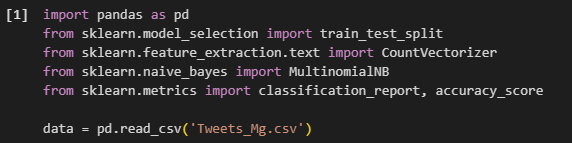
\includegraphics[width=.8\textwidth]{image1.png}
\end{figure}

\begin{figure}[h]
	\centering
	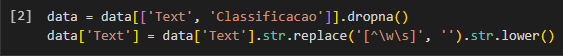
\includegraphics[width=.8\textwidth]{image2.png}
\end{figure}

\begin{figure}[h]
	\centering
	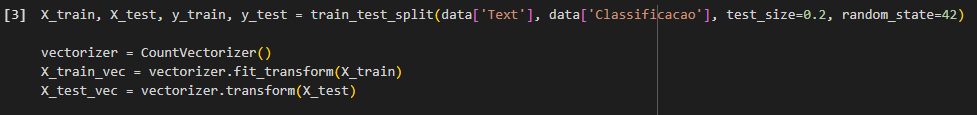
\includegraphics[width=.8\textwidth]{image3.png}
\end{figure}

\begin{figure}[h]
	\centering
	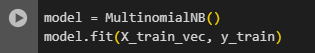
\includegraphics[width=.8\textwidth]{image4.png}
\end{figure}

\begin{figure}[h]
	\centering
	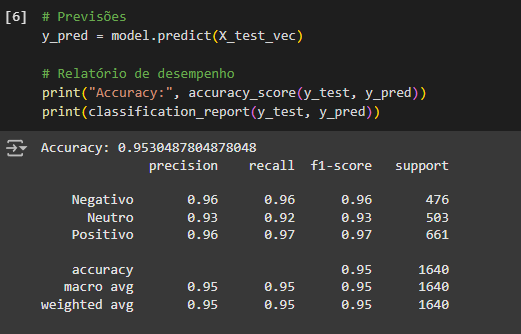
\includegraphics[width=.8\textwidth]{image5.png}
\end{figure}

\end{document}
